\documentclass[11pt]{article}
\usepackage[UTF8]{ctex}

\usepackage[utf8]{inputenc}
\usepackage[T1]{fontenc}
\usepackage{graphicx}
\usepackage{longtable}
\usepackage{wrapfig}
\usepackage{rotating}
\usepackage[normalem]{ulem}
\usepackage{amsmath}
\usepackage{amssymb}
\usepackage{capt-of}
\usepackage{hyperref}
\usepackage[final]{latex/acl}
\usepackage{times}
\usepackage{latexsym}
\usepackage[utf8]{inputenc}
\usepackage{microtype}
\usepackage{inconsolata}
\usepackage{enumitem}
\usepackage{multirow}
\setcounter{secnumdepth}{1}
\date{\today}

\author{
Debarghya Datta \and Soumajit Pramanik \\
Department of Computer Science\\
Indian Institute of Technology, Bhilai\\
\texttt{\{debarghyad,soumajit\}@iitbhilai.ac.in}\\
}

\newcommand{\td}[1]{\textcolor{blue}{[{SP: #1}]}}
\newcommand{\ts}[1]{\textcolor{blue}{[{DD: #1}]}}

\title{低资源领域的无监督命名实体消歧}
\begin{document}
\maketitle
\begin{abstract}
在不断发展的自然语言处理和信息检索领域,对强大且特定领域的实体链接算法的需求变得越发明显。在人文学科、技术写作和生物医学科学等众多领域,丰富文本语义和发现更多知识是至关重要的。在这些领域中使用命名实体消歧 (NED) 需要处理噪声文本、低资源环境和特定领域的知识库 (KBs)。现有的方法大多不适合这种情况,因为它们要么依赖于训练数据,要么不够灵活,无法与领域特定的知识库一起工作。因此,在这项工作中,我们提出了一种利用群体斯坦纳树 (GST) 概念的无监督方法,该方法可以使用文档中所有提及的候选实体之间的上下文相似性来识别实体消歧的最相关候选对象。我们在多个特定领域的数据集上,在Precision@1方面超过当前最先进的无监督方法超过40%(平均)。

\end{abstract}
\section{引言}
命名实体消歧(NED)是通过将文档中的实体提及链接到知识库(KB)中的相应条目来解决实体提及的歧义性任务。最近,NED 已被应用于多个领域,包括数字人文、艺术、建筑、文学和生物医学科学,用于搜索~\cite{meij2014entity}、问答~\cite{yih-etal-2015-semantic}和信息提取~\cite{nooralahzadeh-ovrelid-2018-sirius}等任务。

此类特定领域的 NED 任务的主要挑战有两方面——(a) 它们提供的训练数据很少或没有带有真实标注的数据,(b) 相关的知识图谱(KG)通常很小,并且没有或很少的实体描述~\cite{shi2023knowledge}。为了应对这些挑战,在这项工作中,我们考虑在完全没有标注数据的情况下进行实体消歧。在这种受限的情境下,利用最先进的神经实体链接器变得不可行,因为它们主要依赖于大量的标注数据和足够长的知识图谱中的实体描述~\cite{CadavidSnchez2023EvaluatingEE, arora2021low}。同样,这种设置也排除了无监督的 NED 方法,例如~\cite{pan2015unsupervised},这些方法依赖于标记数据来生成候选实体,如基于领域自适应变压器的模型~\cite{aydin-etal-2022-find}、BLINK~\cite{wu2019zero}、Zeshel~\cite{logeswaran-etal-2019-zero} 和自回归模型如 GENRE~\cite{decao2021autoregressive}。

在文献中,只有少数方法适合我们的受限设置,例如基于图的使用提及距离的方法~\cite{hoffart2011robust}、基于 PageRank/随机游走的方法~\cite{guo2018robust}和基于图排序的方法~\cite{alhelbawy2014graph}。最近~\cite{arora2021low}提出的方法还探索了奇异值分解,展示了低秩子空间中的黄金实体。然而,这些方法在消歧实体时往往难以达到所需的效果。

在这项工作中,我们提出了一种新颖的无监督 NED 方法,用于特定领域的低资源场景,该方法利用了\textbf{群体斯坦纳树}(GSTs)的概念~\cite{garg2000polylogarithmic}。在这种方法中,我们将文档中每个提及的候选实体映射到相关知识图谱中的节点,获取连接这些节点的子图,然后从该子图中提取最小成本的 GSTs。这些 GSTs 通过利用一个事实来促进集体实体消歧,即文档中真正提到的实体(“黄金实体”)往往在文档中所有候选实体的集合中形成一个密集的子图。

\begin{figure*}
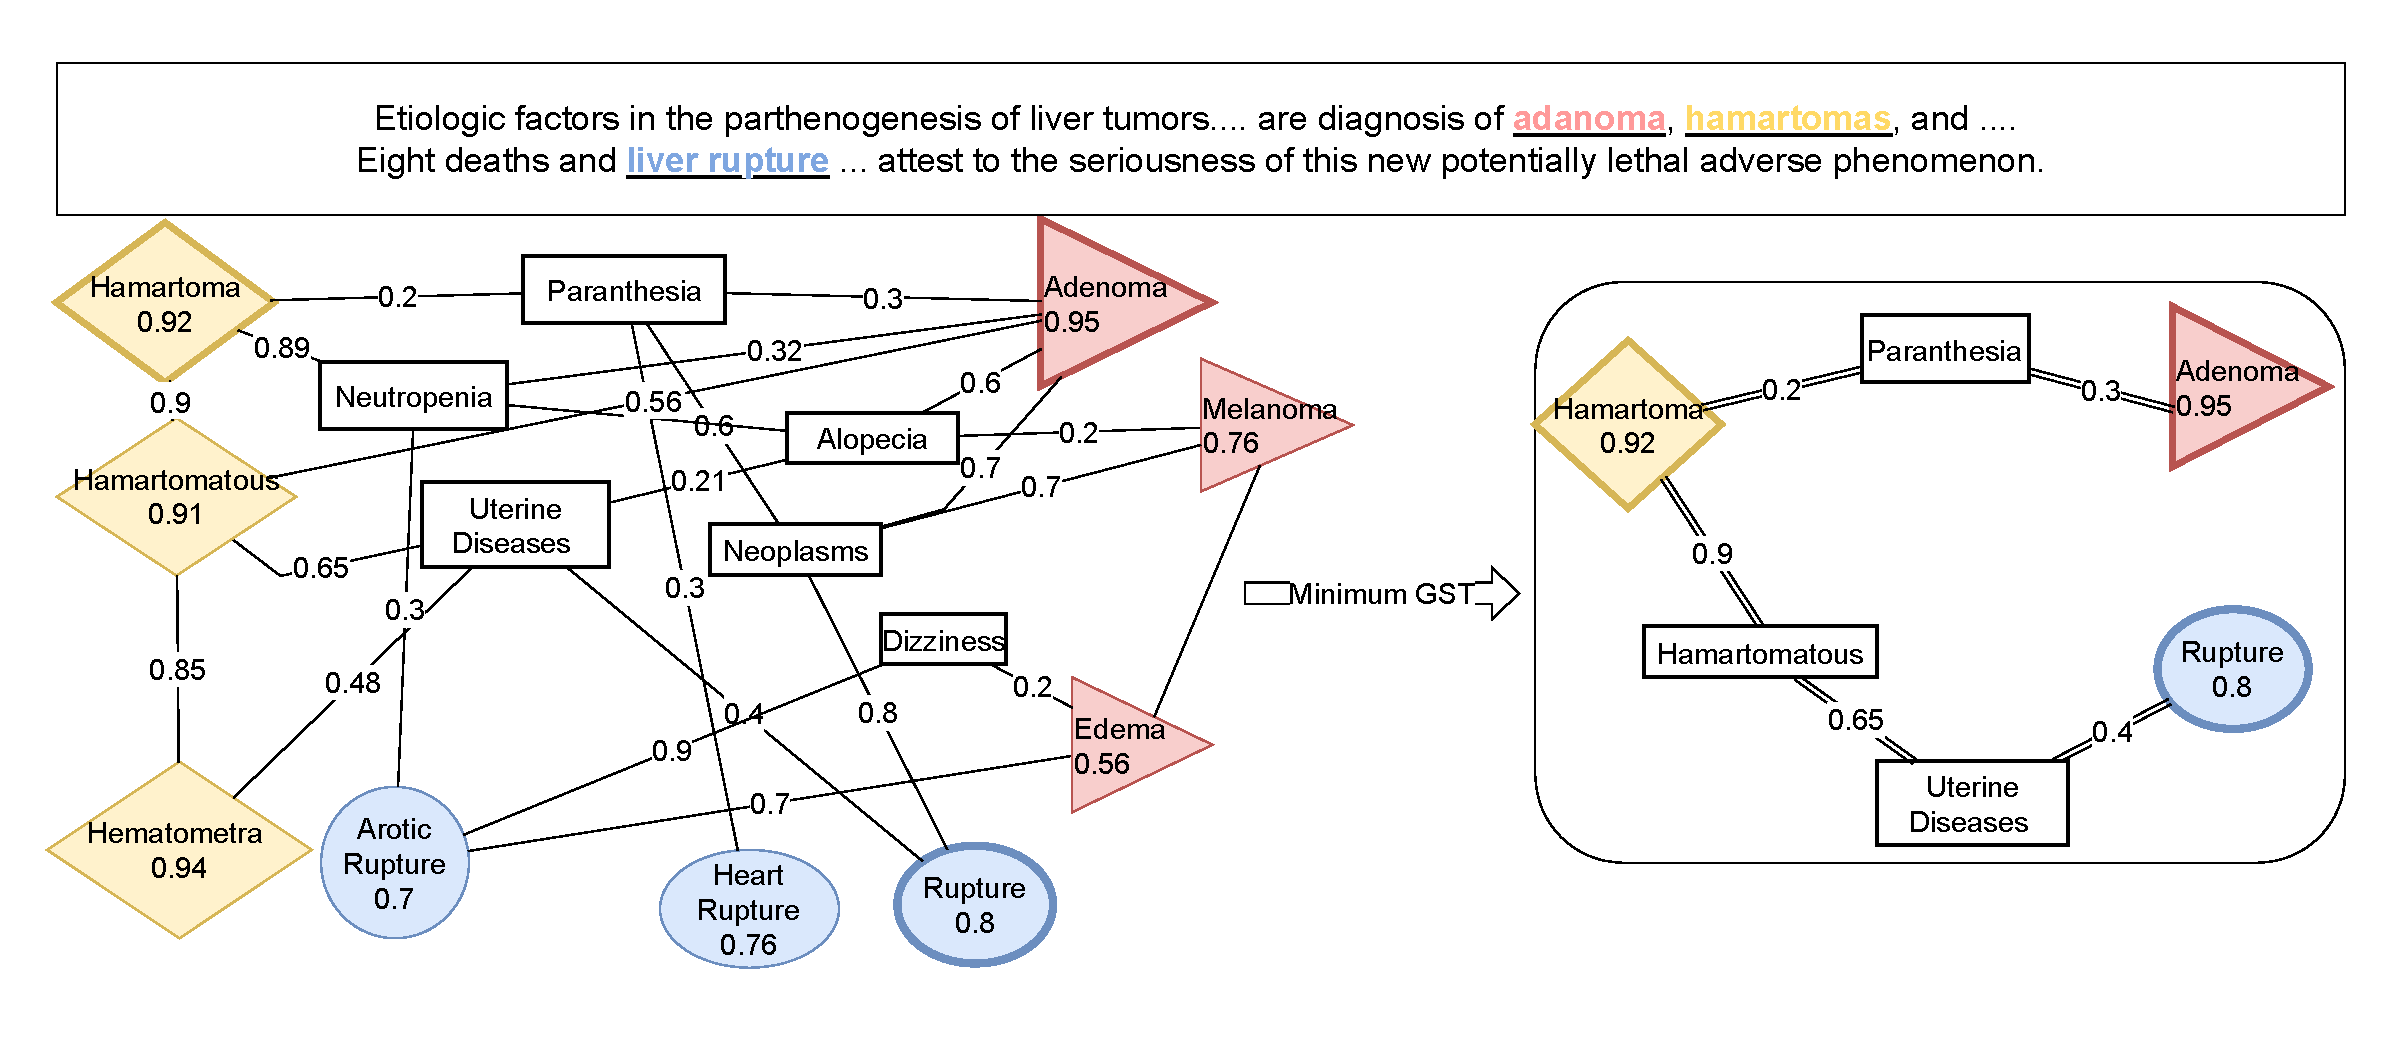
\includegraphics[width=\linewidth]{./pix/pipeline_m4.pdf}
\caption{所提出的 GST-NED 方法:顶部的样本文档包含三个提及;从 KB 中提取的子图显示在左侧,最小成本 GST 使用右侧的框显示。在诱导子图中,`adenoma' 的候选者用红色标记,`hamartomas' 用黄色标记,`liver rupture' 用蓝色标记。}
\label{fig:el-task}
\end{figure*}

总之,我们的主要贡献如下 - (a) 我们提出了一种无监督的\textbf{群体斯坦纳树}(\textbf{GST})\textbf{命名实体消歧}(\textbf{GST-NED})方法,该方法能够在没有标注数据的低资源领域进行 NED;(b) 我们将我们提出的方法与多个领域特定数据集中的几种最先进的基线进行比较,并展示其在各项指标上的显著性能提升(Precision@1 分数平均提高超过 $40\%$)~\footnote{代码可在 \url{https://github.com/deba-iitbh/GST-NED} 获取}。
\section{问题陈述}
与NED文献中的大多数先前工作类似(有少数例外\cite{kolitsas2018end, sil2013re}),我们假设文档级提及范围(通常由命名实体识别器获得)已经提供。设$d$为文档集合$D$中的一个单独文档。另设$M_d = \{m_1, m_2, \ldots , m_M\}$为$d$中包含的$M$个提及的集合,并设$\mathcal{E}$为特定领域知识图谱$KG$中包含的所有实体的集合。这里的任务是为每个提及$m_i$找到其所指的正确实体$e \in \mathcal{E}$。

通常,给定提及集合,一个NED方法通过两个步骤进行消歧——(a) 候选生成,其中从$KG$中为每个提及检索候选实体,(b) 候选排序,其中根据候选实体与相应提及的映射倾向进行排序。在本研究中,我们的主要关注点是候选排序/消歧步骤。接下来,我们描述我们提出的候选排序方法,并提及其他步骤中采用的方法。
\section{方法论}
\subsection{候选生成}
我们索引特定领域的 $KG$,并使用模糊文本搜索 \cite{max_bachmann_2021_5584996} 根据标注提及的表面形式检索候选项。这被认为是最近大多数无监督NED方法中的标准做法~\cite{yang2023b, simos2022computationally}。模糊文本搜索为每个潜在匹配返回一个置信值;我们仅保留置信值超过 $0.75$(经验选择)的候选项~\footnote{如果与KG节点完全匹配,我们认为这是提及的正确匹配,并跳过候选排名步骤。}。
\subsection{候选排名}

我们使用知识图($KG$)为特定文档 $d$ 中从候选生成步骤获得的所有候选实体对创建一个子图。为了保持图的规模可控,我们将路径长度限制为实体候选之间最多三跳。我们进一步通过基于Jaro-Winkler距离~\cite{wang2017efficient}(反映候选与提及的相似性)添加节点权重,以及基于节点2Vec \cite{grover2016node2vec}结构嵌入的端点余弦相似性添加边权重来增强图。在图~\ref{fig:el-task} 中,我们展示了一个具有三个提及的文档及其相应的候选实体诱导子图(左侧)。

\noindent
\textbf{寻找GST:}我们识别正确候选实体的方法依赖于这样的直觉:文档 $d$ 中的一个黄金实体候选应该在诱导子图中比其他非黄金候选与其他黄金候选连接得更紧密。换句话说,我们期望在诱导子图中的黄金实体由于其上下文接近性(因为它们在同一个文档中使用)形成紧密相连的子图。为了利用这一直觉,我们首先定义终端的概念——对于每个提及 $m_i$,我们将相应的候选实体节点标记为该提及的终端节点,并将它们分组为 $T_i$。接下来任务是从每个终端组中选择正确的候选节点,为此我们利用了组斯坦纳树(GST)的概念~\cite{ding2006finding,pramanik2024uniqorn},定义如下, \begin{itemize}[topsep=2pt,itemsep=0pt,partopsep=0pt, parsep=0pt]
\item 给定一个无向加权图 \((V, E)\) 以及一组终端节点 \(\{T_1, . . . ,T_l\}\),其中每个 \(T_\nu \subseteq V\),计算连接 \(\{T_1, . . . ,T_l\}\) 中至少一个节点的最小代价树 \((V^*, E^*)\):\(\min \sum_{ij \in E^*} c_{ij}\) ,满足 \(T_\nu \cap V^* \ne \emptyset, \ \forall T_\nu\)。
\end{itemize} 在我们的情况下,我们考虑 $c_{ij}=(1 - w_{ij})$,其中 $w_{ij}$ 表示节点 $i$ 和 $j$ 之间的边权重。如定义所述,每个GST必须至少选择每个终端组中的一个候选实体。因此,每个检测到的GST将至少提供一个潜在的实体消歧问题的解决方案。由于我们进一步假设黄金候选实体比非黄金候选连接得更紧密,因此增加了在最低成本GST中被选择的黄金候选的概率(因为最低成本GST确保了所选候选之间的距离较短且边权重较高,即边成本较低)。例如,在图~\ref{fig:el-task} 的右侧,我们展示了从诱导子图中提取的最低成本GST包含了所有对应于文档中提及的黄金候选实体。

\noindent
\textbf{放宽到GST-k和排名标准}: 在我们的设置中,我们实际上寻找的是从k个最低成本GST中提取的实体候选(在我们的工作中经验性地使用了k=10),而不是仅依赖于最低成本GST。这是为了增强方法的鲁棒性,因为它允许我们有效地排名不同的候选实体。我们利用以下三种直观的排名方案为每个提及的候选实体排名,并选择排名较高的实体 - \textbf{(a) GST计数}:候选出现的GST数量;越多越好,\textbf{(b) GST成本}:候选出现的GST总成本;越低越好,以及 \textbf{(c) 节点权重:} 候选出现的GST中的节点权重之和;越高越好。随后,我们比较所有三种方案的表现以选择最佳方案。

\noindent
\textbf{复杂性:}斯坦纳树是经典的NP完全问题之一~\cite{ding2006finding},这同样适用于GST问题。然而,当将终端数视为常数时,该问题具有可处理的固定参数复杂性 \cite{downey2013fundamentals},并且在数据库关键词搜索领域广泛应用了良好的多项式时间近似算法 \cite{ding2006finding,kacholia2005bidirectional,li2016efficient}。在\emph{GST-NED} 中,我们基于 \cite{ding2006finding} 的精确解法,该方法采用动态规划方法,在提及数(通常有限)上具有指数运行时间,但在图规模上具有 $O(n\log n)$ 复杂性。
\section{实验设置}
\subsection{数据集}
为了展示我们模型的有效性,我们选择了来自文学、法律、博物馆文物和化学品等不同领域的以下四个数据集(更多详细信息见表~\ref{tab:data-stat})。

\noindent
\textbf{WWO}\footnote{\url{https://www.wwp.northeastern.edu/wwo}} 是一个由维多利亚时代前女性作家创作的文本文档(诗歌、戏剧和小说)组成的集合,部分标注了人物、作品和地点实体~\cite{flanders2010encoding}。

\begin{table}
\resizebox{\columnwidth}{!}{
\begin{tabular}{lrrrrrr}
Dataset & \#D & \#M & \#N & \#E & \#C & \#R\\[0pt]
\hline
WWO & 76 & 14651 & 9065 & 4936 & 10 & 0.83\\[0pt]
1641 & 16 & 480 & 3503 & 338 & 10 & 0.26\\[0pt]
Artifact & 168 & 6311 & 41180 & 42634 & 11 & 0.66\\[0pt]
Chemical & 135 & 15769 & 176415 & 249275 & 10 & 0.73\\[0pt]
\end{tabular}
}
\caption{\label{tab:data-stat}四个使用数据集的数据统计:文档总数 ($\#D$)、提及总数 ($\#M$)、知识图谱中的节点数 ($\#N$) 和边数 ($\#E$)、每个提及的平均候选数 ($\#C$) 以及候选实体的召回率,即在候选项中具有黄金实体的提及比例 ($\#R$)}.
\end{table}

\noindent
\textbf{1641}\footnote{\url{http://1641.tcd.ie/}} 包含记录在1641年爱尔兰叛乱后法庭证人陈述形式的法律文本,部分标注了与DBpedia知识库子集对比的人名~\cite{klie2020zero}。

\noindent
\textbf{Chemical} 数据集来自BC5CDR语料库 ~\cite{li2016biocreative}。它包含了化学品的全面人工标注,每个化学品都有独特的MeSH标识符。化学品的分类使用了来自比较毒理基因组学数据库(CTD)~\footnote{\url{https://www.ctdbase.org/}} 的化学品词汇。

\noindent
\textbf{Artifact}~\cite{CadavidSnchez2023EvaluatingEE} 是一个博物馆对象的数字描述集合,标注了四个不同的文本字段:标题、详细描述、对Getty艺术及建筑词表~\footnote{\url{https://www.getty.edu/research/tools/vocabularies/aat/about.html}}(AAT)的自由形式元数据。
\subsection{基线}
为了比较我们提出方法的性能,我们利用以下基线\footnote{所有数据集和基线代码均可在MIT \& Apache许可证下获得。}。

\noindent
\textbf{NameMatch}\cite{klie2020zero}。我们采用字符串匹配的方法来选择与提及的表面形式完全匹配的候选项。

\noindent
\textbf{BLINK*}~\cite{wu2019zero}。我们在领域特定设置中调整了一个微调的BLINK模型,用于预测每个提及的命名实体。由于默认情况下它将实体匹配到维基百科\footnote{\url{https://www.wikipedia.org/}},我们随后进行模糊匹配过程,以将预测的实体与我们领域特定的知识库对齐。

\noindent
\textbf{WalkingNED}~\cite{guo2018robust} 是一种基于图的方式,用于基于局部相似性(表面形式相似性)和全局相似性(候选项的语义签名与文档之间的相似性,通过PageRank计算)来消除提及候选项的歧义。

\noindent
\textbf{Eigenthemes}~\cite{arora2021low} 是一种方法,利用“黄金实体”在嵌入空间内聚集在一起的固有性质,通过将实体表示为向量并利用奇异值分解(SVD)。 

\begin{table}[htbp]
\centering
\begin{tabular}{p{2cm}p{2cm}p{1cm}p{1cm}}
Dataset & Model & P@1 & HIT@5\\[0pt]
\hline
 WWO
 & NameMatch	& 0.35 & 0.35 \\
 & BLINK* & 0.07 & 0.09 \\
 & WalkingNED & 0.18 & 0.49\\
 & EigenThemes & 0.14 & 0.45\\
 & GST-NED & \textbf{0.57} & \textbf{0.72}\\
\hline
 1641
 & NameMatch & 0.06 & 0.06 \\
 & BLINK* & 0.05	& 0.11 \\
 & WalkingNED & 0.11 & 0.17\\
 & EigenThemes & 0.17 & \textbf{0.25}\\
 & GST-NED & \textbf{0.20} & 0.22 \\
\hline
Artifact
 & NameMatch & 0.23 & 0.23 \\
 & BLINK* & 0.02	& 0.03 \\
 & WalkingNED & 0.26 & 0.56\\
 & EigenThemes & 0.15 & 0.44\\
 & GST-NED & \textbf{0.54} & \textbf{0.61} \\
\hline
 Chemical
 & NameMatch	& 0.08 & 0.08 \\
 & BLINK* & 0.13 & 0.22 \\
 & WalkingNED & 0.50 & \textbf{0.66}\\
 & EigenThemes & 0.36 & 0.59\\
 & GST-NED & \textbf{0.52} & \textbf{0.66}\\
 \hline
\end{tabular}
\caption{\label{tab:org1c6e60d} NED 性能比较:WWO、1641、Artifact 和 Chemical 数据集。}
\end{table}
\subsection{指标}
与 NED 领域的最新文献类似,我们使用 Precision@1(最高排名候选的正确性)和 Hit@5(前五名排名候选中存在金标实体)作为我们的评估指标。
\section{结果与讨论}
我们将提出的 \emph{GST-NED} 方法与其他基线算法进行了比较,相应的结果如表~\ref{tab:org1c6e60d} 所示。我们可以观察到,我们的方法在所有数据集上(尤其是在 $P@1$ 方面)优于现有的最先进技术。在 1641 数据集中,所有算法表现相对较差的原因在于候选实体的召回率较低(参见表~\ref{tab:data-stat})。总体而言,BLINK* 表现不佳,因为它难以在特定领域的知识库中找到合适的匹配。

\begin{table}[htbp]
    \centering
    \begin{tabular}{c|c|c}
     & WWO	& Artifact \\
    \hline
    GST count	& \textbf{0.57} & \textbf{0.54} \\
    GST cost	& 0.55 & 0.51 \\
    Node weight	& 0.54 & 0.53 \\
    \end{tabular}
    \caption{在两个数据集上排名方案的比较 (P@1)}
    \label{tab:abl_tab}
\end{table}

\noindent
\textbf{排名方案分析}
在表~\ref{tab:abl_tab} 中,我们分析了在 $\emph{GST-NED}$ 中选择不同的候选排名方案的影响。观察到 GST-count 方案在我们的场景中表现最佳。

\noindent
\textbf{参数微调}
为了优化指标值,我们进行了广泛的实证实验,调整了候选生成的模糊阈值和候选排名中不同数量的前 k 名 GST。这些实验在 'WWO' 和 'Artifact' 数据集的一个小型保留子集(约 $10\%$)上进行,结果如表~\ref{tbl:hyper_threshold}、\ref{tbl:hyper_k} 所示。根据我们的分析,考虑 $0.75$ 的模糊阈值和前 10 个 GST 能够在我们的设置中获得最高的 Precision@1 分数。因此,这些参数被用于本文报告的所有实验。

\begin{table}[htbp]
\centering
\begin{tabular}{c|cc}
Threshold & WWO & Artifact \\ \hline
0.70 & 0.632 & 0.574 \\
0.75 & 0.634 & 0.580 \\
0.80 & 0.632 & 0.562 \\
0.85 & 0.631 & 0.554 \\
0.90 & 0.633 & 0.554 \\
\end{tabular}
\caption{\label{tbl:hyper_threshold}不同模糊匹配阈值下,保留的 WWO 和 Artifact 数据集的 Precision@1}
\end{table}

\begin{table}[htbp]
\centering
\begin{tabular}{c|cc}
k & WWO & Artifact \\ \hline
1  & 0.63 & 0.55 \\
5  & 0.63 & 0.57 \\
10 & 0.64 & 0.58 \\
20 & 0.62 & 0.56 \\
50 & 0.63 & 0.56 \\
\end{tabular}
\caption{\label{tbl:hyper_k}在不同的 $k$ (排名靠前的 GST 数量)值下,保留的 WWO 和 Artifact 数据集的 Precision@1}
\end{table}
\noindent
\textbf{错误分析}
我们进行了详细的错误分析,以确定我们提出的流程中错误的分布情况。具体来说,我们计算了由于以下原因导致错误的实例比例:(a)候选列表中不存在黄金(正确)实体,(b)黄金实体存在于候选列表中但不在前 k 个 GST 中,(c)黄金实体包含在前 k 个 GST 中但未排在前 1 位。在 'WWO' 数据集中,14\% 的错误属于(a),11\% 属于(b),18\% 属于(c),其余 57\% 的情况得到正确解决,precision@1 分数为 0.57。这些发现表明,加强排名机制和候选生成过程对于实现性能提升至关重要。
\section{结论}
在本文中,我们解决了在缺乏标注数据的情况下对特定领域语料库进行命名实体识别的问题。其工作原理基于这样一个直觉:来自文档的一个黄金实体候选应该在知识图谱中与其他黄金候选相比于非黄金候选有更紧密的联系。我们利用了群体斯坦纳树(Group Steiner Trees, GSTs)的概念,该概念仅依赖于候选实体名称和特定领域知识图谱的可用性。在我们提出的方法\emph{GST-NED}中提取最小成本GSTs,确保所选实体在特定领域知识图谱中紧密相连。对来自不同领域的基准数据集的实验表明,我们提出的方法在对比当前最先进的无监督和零样本方法时具有有效性。
\section*{局限性}
我们的实体消歧方法,\emph{GST-NED},依赖于每个文档中存在足够数量的实体以准确地运行,因为我们依靠实体的联合消歧。因此,当实体数量非常少时,它无法提供正确的响应。另一方面,考虑包含过多实体的相对较长的文档块会增加图的大小,从而影响我们的计算效率。因此,有必要通过详细和彻底的研究来分析这一权衡。有趣的是,考虑较长的文档也增加了同一提及多次使用不同含义的可能性,而这超出了我们模型目前的能力范围。

\noindent 此外,还需要进一步的工作来提高我们用于计算最优树的斯坦纳树算法的可扩展性。目前,对于像WWO、1641或Artifact这样的小型知识图谱,每个文档大约需要2秒,而在化学数据集的相对较大的知识图谱上,每个文档大约需要40秒(在具有$3.9$GHz CPU和$16$ GB RAM的系统上)。
\section*{伦理}
本工作中的数据和模型是公开可用的。它们可能包含偏见,应谨慎使用。

\bibliography{acl_latex}

\end{document}
